\documentclass[10pt]{article}
\usepackage[polish]{babel}
\usepackage[utf8]{inputenc}
\usepackage[T1]{fontenc}
\usepackage{graphicx}
\usepackage[export]{adjustbox}
\graphicspath{ {./images/} }
\usepackage{amsmath}
\usepackage{amsfonts}
\usepackage{amssymb}
\usepackage[version=4]{mhchem}
\usepackage{stmaryrd}
\usepackage{multirow}

\newcommand\Varangle{\mathop{{<\!\!\!\!\!\text{\small)}}\:}\nolimits}

\begin{document}
Klasa ............\\
Nazwisko i imię\\
PRÓBNY EGZAMIN MATURALNY Z MATEMATYKI\\

\includegraphics[max width=\textwidth, center]{2024_11_21_49bfa1d51da2e7fce9c5g-01}

\section*{Instrukcja dla zdającego}
\begin{enumerate}
  \item Sprawdź, czy arkusz egzaminacyjny zawiera 16 stron (zadania 1-15).\\
Ewentualny brak zgłoś przewodniczącemu zespołu nadzorującego egzamin.
  \item Rozwiązania zadań i odpowiedzi wpisuj w miejscu na to przeznaczonym.
  \item Odpowiedzi do zadań zamkniętych (1-4) przenieś do tabelki odpowiedzi, a w zadaniu 5 zakoduj odpowiedź zgodnie z instrukcją zapisaną w treści zadania.
  \item Pamiętaj, że pominięcie argumentacji lub istotnych obliczeń w rozwiązaniu zadania otwartego (6-15) może spowodować, że za to rozwiązanie nie otrzymasz pełnej liczby punktów.
  \item Pisz czytelnie i używaj tylko długopisu lub pióra z czarnym tuszem lub atramentem.
  \item Nie używaj korektora, a błędne zapisy wyraźnie przekreśl.
  \item Pamiętaj, że zapisy w brudnopisie nie będą oceniane.
  \item Możesz korzystać z zestawu wzorów matematycznych, cyrkla i linijki oraz kalkulatora prostego.
\end{enumerate}

Życzymy powodzenia!

MARZEC\\
ROK 2020

Za rozwiązanie\\
wszystkich zadań\\
można otrzymać\\
łącznie\\
50 punktów

\section*{ZADANIA ZAMKNIĘTE}
\section*{W zadaniach od 1. do 4. wybierz i wpisz w tabelce poprawnq odpowiedź.}
\begin{center}
\begin{tabular}{|c|c|c|c|c|}
\hline
Nrzadania & 1 & 2 & 3 & 4 \\
\hline
Zaznaczona odpowiedź &  &  &  &  \\
\hline
\end{tabular}
\end{center}

\section*{Zadanie 1. (0-1)}
Okrąg o równaniu \((x+8)^{2}+(y+4)^{2}=25\) jest styczny wewnętrznie do okręgu o środku \(S=(0,2)\) i promieniu \(r\), zatem\\
A. \(r=10\)\\
B. \(r=15\)\\
C. \(r=5\)\\
D. \(r=20\)

\section*{Zadanie 2. (0-1)}
Liczba \(2 \log _{9} 15-\frac{1}{2} \log _{\sqrt{3}} 5\) jest równa\\
A. 0\\
B. 3\\
C. \(\frac{1}{3}\)\\
D. 1

\section*{Zadanie 3. (0-1)}
Reszta z dzielenia wielomianu \(W(x)=a x^{3}-x^{2}+3\) przez dwumian \(x+2\) jest równa 3 , zatem\\
A. \(a=\frac{1}{2}\)\\
B. \(a=\frac{1}{8}\)\\
C. \(a=-\frac{1}{2}\)\\
D. \(a=-\frac{1}{8}\)

\section*{Zadanie 4. (0-1)}
Równanie \(\sin 3 x+2 \cos 4 x=4\) w przedziale \((-\pi ; \pi)\)\\
A. nie ma rozwiązań rzeczywistych\\
B. ma dokładnie cztery rozwiązania rzeczywiste\\
C. ma dokładnie dwa rozwiązania rzeczywiste\\
D. ma dokładnie trzy rozwiązania rzeczywiste

\section*{Zadanie 5. (0-2)}
Dane są zdarzenia losowe \(A, B \subset \Omega\) takie, że \(P\left(B^{\prime}\right)=\frac{1}{3} \quad\) i \(P(A \cup B)=\frac{4}{5}\). Oblicz \(P(A \backslash B)\), gdzie zdarzenie \(A \backslash B\) oznacza różnicę zdarzeń \(A\) i \(B\). Zakoduj kolejno pierwsze trzy cyfry po przecinku rozwinięcia dziesiętnego otrzymanego wyniku.\\
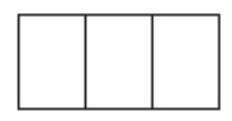
\includegraphics[max width=\textwidth, center]{2024_11_21_49bfa1d51da2e7fce9c5g-02}

BRUDNOPIS (nie podlega ocenie)\\

\includegraphics[max width=\textwidth, center]{2024_11_21_49bfa1d51da2e7fce9c5g-03}

\section*{Zadanie 6. (0-3)}
W trójkącie \(A B C\) długośsi boków spełniają warunki: \(|B C|=14,|A B|=2|A C|\) oraz miara kąta wewnętrznego \(B A C\) jest równa \(120^{\circ}\). Oblicz obwód tego trójkąta.

\begin{center}
\begin{tabular}{|c|c|c|c|c|c|c|c|c|c|c|c|c|c|c|c|c|c|c|c|c|c|c|c|c|c|c|c|}
\hline
 &  &  &  &  &  &  &  &  &  &  &  &  &  &  &  &  &  &  &  &  &  &  &  &  &  &  &  \\
\hline
 &  &  &  &  &  &  &  &  &  &  &  &  &  &  &  &  &  &  &  &  &  &  &  &  &  &  &  \\
\hline
 &  &  &  &  &  &  &  &  &  &  &  &  &  &  &  &  &  &  &  &  &  &  &  &  &  &  &  \\
\hline
 &  &  &  &  &  &  &  &  &  &  &  &  &  &  &  &  &  &  &  &  &  &  &  &  &  &  &  \\
\hline
 &  &  &  &  &  &  &  &  &  &  &  &  &  &  &  &  &  &  &  &  &  &  &  &  &  &  &  \\
\hline
 &  &  &  &  &  &  &  &  &  &  &  &  &  &  &  &  &  &  &  &  &  &  &  &  &  &  &  \\
\hline
 &  &  &  &  &  &  &  &  &  &  &  &  &  &  &  &  &  &  &  &  &  &  &  &  &  &  &  \\
\hline
 &  &  &  &  &  &  &  &  &  &  &  &  &  &  &  &  &  &  &  &  &  &  &  &  &  &  &  \\
\hline
 &  &  &  &  &  &  &  &  &  &  &  &  &  &  &  &  &  &  &  &  &  &  &  &  &  &  &  \\
\hline
 &  &  &  &  &  &  &  &  &  &  &  &  &  &  &  &  &  &  &  &  &  &  &  &  &  &  &  \\
\hline
 &  &  &  &  &  &  &  &  &  &  &  &  &  &  &  &  &  &  &  &  &  &  &  &  &  &  &  \\
\hline
 &  &  &  &  &  &  &  &  &  &  &  &  &  &  &  &  &  &  &  &  &  &  &  &  &  &  &  \\
\hline
 &  &  &  &  &  &  &  &  &  &  &  &  &  &  &  &  &  &  &  &  &  &  &  &  &  &  &  \\
\hline
 &  &  &  &  &  &  &  &  &  &  &  &  &  &  &  &  &  &  &  &  &  &  &  &  &  &  &  \\
\hline
 &  &  &  &  &  &  &  &  &  &  &  &  &  &  &  &  &  &  &  &  &  &  &  &  &  &  &  \\
\hline
 &  &  &  &  &  &  &  &  &  &  &  &  &  &  &  &  &  &  &  &  &  &  &  &  &  &  &  \\
\hline
 &  &  &  &  &  &  &  &  &  &  &  &  &  &  &  &  &  &  &  &  &  &  &  &  &  &  &  \\
\hline
 &  &  &  &  &  &  &  &  &  &  &  &  &  &  &  &  &  &  &  &  &  &  &  &  &  &  &  \\
\hline
 &  &  &  &  &  &  &  &  &  &  &  &  &  &  &  &  &  &  &  &  &  &  &  &  &  &  &  \\
\hline
 &  &  &  &  &  &  &  &  &  &  &  &  &  &  &  &  &  &  &  &  &  &  &  &  &  &  &  \\
\hline
 &  &  &  &  &  &  &  &  &  &  &  &  &  &  &  &  &  &  &  &  &  &  &  &  &  &  &  \\
\hline
 &  &  &  &  &  &  &  &  &  &  &  &  &  &  &  &  &  &  &  &  &  &  &  &  &  &  &  \\
\hline
 & - &  &  &  &  &  &  &  &  &  &  &  &  &  &  &  &  &  &  &  &  &  &  &  &  &  &  \\
\hline
 &  &  &  &  &  &  &  &  &  &  &  &  &  &  &  &  &  &  &  &  &  &  &  &  &  &  &  \\
\hline
 & \(\square\) &  &  &  &  &  &  &  &  &  &  &  &  &  &  &  &  &  &  &  &  &  &  &  &  &  &  \\
\hline
 & 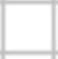
\includegraphics[max width=\textwidth]{2024_11_21_49bfa1d51da2e7fce9c5g-04}
 &  &  &  &  &  &  &  &  &  &  &  &  &  &  &  &  &  &  &  &  &  &  &  &  &  &  \\
\hline
 &  &  &  &  &  &  &  &  &  &  &  &  &  &  &  &  &  &  &  &  &  &  &  &  &  &  &  \\
\hline
 & \textbackslash  &  &  &  &  &  &  &  &  &  &  &  &  &  &  &  &  &  &  &  &  &  &  &  &  &  &  \\
\hline
 & - &  &  &  &  &  &  &  &  &  &  &  &  &  &  &  &  &  &  &  &  &  &  &  &  &  &  \\
\hline
 &  &  &  &  &  &  &  &  &  &  &  &  &  &  &  &  &  &  &  &  &  &  &  &  &  &  &  \\
\hline
 &  &  &  &  &  &  &  &  &  &  &  &  &  &  &  &  &  &  &  &  &  &  &  &  &  &  &  \\
\hline
 &  &  &  &  &  &  &  &  &  &  &  &  &  &  &  &  &  &  &  &  &  &  &  &  &  &  &  \\
\hline
 &  &  &  &  &  &  &  &  &  &  &  &  &  &  &  &  &  &  &  &  &  &  &  &  &  &  &  \\
\hline
 &  &  &  &  &  &  &  &  &  &  &  &  &  &  &  &  &  &  &  &  &  &  &  &  &  &  &  \\
\hline
 &  &  &  &  &  &  &  &  &  &  &  &  &  &  &  &  &  &  &  &  &  &  &  &  &  &  &  \\
\hline
 &  &  &  &  &  &  &  &  &  &  &  &  &  &  &  &  &  &  &  &  &  &  &  &  &  &  &  \\
\hline
 &  &  &  &  &  &  &  &  &  &  &  &  &  &  &  &  &  &  &  &  &  &  &  &  &  &  &  \\
\hline
\end{tabular}
\end{center}

Odpowiedź: \(\qquad\)

\begin{center}
\begin{tabular}{|c|l|c|}
\hline
\multirow{2}{*}{\begin{tabular}{c}
Wypełnia \\
egzaminator \\
\end{tabular}} & Nr zadania & 6. \\
\cline { 2 - 3 }
 & Maks. liczba pkt. & 3 \\
\cline { 2 - 3 }
 & Uzyskana liczba pkt. &  \\
\hline
\end{tabular}
\end{center}

Zadanie 7. (0-3)\\
Rozwiąż równanie \(2 \cos ^{2} x=-3 \sin x\) w przedziale \(\langle-\pi ; 2 \pi\rangle\).\\

\includegraphics[max width=\textwidth, center]{2024_11_21_49bfa1d51da2e7fce9c5g-05}

Odpowiedź: \(\qquad\)

\begin{center}
\begin{tabular}{|c|l|c|}
\hline
\multirow{2}{*}{\begin{tabular}{c}
Wypełnia \\
egzaminator \\
\end{tabular}} & Nr zadania & 7. \\
\cline { 2 - 3 }
 & Maks. liczba pkt. & 3 \\
\cline { 2 - 3 }
 & Uzyskana liczba pkt. &  \\
\hline
\end{tabular}
\end{center}

\section*{Zadanie 8. (0-3)}
Na boku \(A B\) trójkąta \(A B C\) obrano punkt \(D\) w ten sposób, że \(\frac{|A D|}{|D B|}=\frac{2}{3}\). Na odcinku \(C D\) obrano taki punkt \(F\), że \(\frac{|D F|}{|D C|}=\frac{1}{4}\) (popatrz na rysunek). Przez punkty \(B\) i \(F\) poprowadzono prostą, która przecięła bok \(A C\) w punkcie \(E\). Uzasadnij, że stosunek pola trójkąta \(A E B\) do pola trójkąta ECB jest równy 5: 9.\\
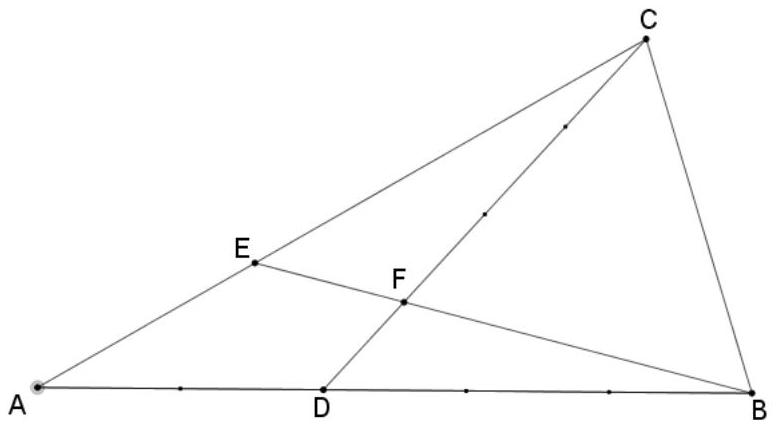
\includegraphics[max width=\textwidth, center]{2024_11_21_49bfa1d51da2e7fce9c5g-06}

\begin{center}
\begin{tabular}{|c|c|c|c|c|c|c|c|c|c|c|c|c|c|c|c|c|c|c|c|c|c|c|c|c|c|c|c|c|c|c|}
\hline
 &  &  &  &  &  &  &  &  &  &  &  &  &  &  &  &  &  &  &  &  &  &  &  &  &  &  &  &  &  &  \\
\hline
 &  &  &  &  &  &  &  &  &  &  &  &  &  &  &  &  &  &  &  &  &  &  &  &  &  &  &  &  &  &  \\
\hline
 &  &  &  &  &  &  &  &  &  &  &  &  &  &  &  &  &  &  &  &  &  &  &  &  &  &  &  &  &  &  \\
\hline
 &  &  &  &  &  &  &  &  &  &  &  &  &  &  &  &  &  &  &  &  &  &  &  &  &  &  &  &  &  &  \\
\hline
 &  &  &  &  &  &  &  &  &  &  &  &  &  &  &  &  &  &  &  &  &  &  &  &  &  &  &  &  &  &  \\
\hline
 &  &  &  &  &  &  &  &  &  &  &  &  &  &  &  &  &  &  &  &  &  &  &  &  &  &  &  &  &  &  \\
\hline
 &  &  &  &  &  &  &  &  &  &  &  &  &  &  &  &  &  &  &  &  &  &  &  &  &  &  &  &  &  &  \\
\hline
 &  &  &  &  &  &  &  &  &  &  &  &  &  &  &  &  &  &  &  &  &  &  &  &  &  &  &  &  &  &  \\
\hline
 &  &  &  &  &  &  &  &  &  &  &  &  &  &  &  &  &  &  &  &  &  &  &  &  &  &  &  &  &  &  \\
\hline
 &  &  &  &  &  &  &  &  &  &  &  &  &  &  &  &  &  &  &  &  &  &  &  &  &  &  &  &  &  &  \\
\hline
 &  &  &  &  &  &  &  &  &  &  &  &  &  &  &  &  &  &  &  &  &  &  &  &  &  &  &  &  &  &  \\
\hline
 &  &  &  &  &  &  &  &  &  &  &  &  &  &  &  &  &  &  &  &  &  &  &  &  &  &  &  &  &  &  \\
\hline
 &  &  &  &  &  &  &  &  &  &  &  &  &  &  &  &  &  &  &  &  &  &  &  &  &  &  &  &  &  &  \\
\hline
 &  &  &  &  &  &  &  &  &  &  &  &  &  &  &  &  &  &  &  &  &  &  &  &  &  &  &  &  &  &  \\
\hline
 &  &  &  &  &  &  &  &  &  &  &  &  &  &  &  &  &  &  &  &  &  &  &  &  &  &  &  &  &  &  \\
\hline
 &  &  &  &  &  &  &  &  &  &  &  &  &  &  &  &  &  &  &  &  &  &  &  &  &  &  &  &  &  &  \\
\hline
 &  &  &  &  &  &  &  &  &  &  &  &  &  &  &  &  &  &  &  &  &  &  &  &  &  &  &  &  &  &  \\
\hline
 &  &  &  &  &  &  &  &  &  &  &  &  &  &  &  &  &  &  &  &  &  &  &  &  &  &  &  &  &  &  \\
\hline
 &  &  &  &  &  &  &  &  &  &  &  &  &  &  &  &  &  &  &  &  &  &  &  &  &  &  &  &  &  &  \\
\hline
 &  &  &  &  &  &  &  &  &  &  &  &  &  &  &  &  &  &  &  &  &  &  &  &  &  &  &  &  &  &  \\
\hline
 &  &  &  &  &  &  &  &  &  &  &  &  &  &  &  &  &  &  &  &  &  &  &  &  &  &  &  &  &  &  \\
\hline
 &  &  &  &  &  &  &  &  &  &  &  &  &  &  &  &  &  &  &  &  &  &  &  &  &  &  &  &  &  &  \\
\hline
 &  &  &  &  &  &  &  &  &  &  &  &  &  &  &  &  &  &  &  &  &  &  &  &  &  &  &  &  &  &  \\
\hline
 &  &  &  &  &  &  &  &  &  &  &  &  &  &  &  &  &  &  &  &  &  &  &  &  &  &  &  &  &  &  \\
\hline
 & - &  &  &  &  &  &  &  &  &  &  &  &  &  &  &  &  &  &  &  &  &  &  &  &  &  &  &  &  &  \\
\hline
 &  &  &  &  &  &  &  &  &  &  &  &  &  &  &  &  &  &  &  &  &  &  &  &  &  &  &  &  &  &  \\
\hline
\end{tabular}
\end{center}

Odpowiedź: \(\qquad\)

\begin{center}
\begin{tabular}{|c|l|c|}
\hline
\multirow{2}{*}{\begin{tabular}{c}
Wypełnia \\
egzaminator \\
\end{tabular}} & Nr zadania & 8. \\
\cline { 2 - 3 }
 & Maks. liczba pkt. & 3 \\
\cline { 2 - 3 }
 & Uzyskana liczba pkt. &  \\
\hline
\end{tabular}
\end{center}

BRUDNOPIS (nie podlega ocenie)

\begin{center}
\begin{tabular}{|c|c|c|c|c|c|c|c|c|c|c|c|c|c|c|c|c|c|c|c|c|c|c|c|c|c|c|c|c|c|c|c|}
\hline
 &  &  &  &  &  &  &  &  &  &  &  &  &  &  &  &  &  &  &  &  &  &  &  &  &  &  &  &  &  &  &  \\
\hline
 &  &  &  &  &  &  &  &  &  &  &  &  &  &  &  &  &  &  &  &  &  &  &  &  &  &  &  &  &  &  &  \\
\hline
 &  &  &  &  &  &  &  &  &  &  &  &  &  &  &  &  &  &  &  &  &  &  &  &  &  &  &  &  &  &  &  \\
\hline
 &  &  &  &  &  &  &  &  &  &  &  &  &  &  &  &  &  &  &  &  &  &  &  &  &  &  &  &  &  &  &  \\
\hline
 &  &  &  &  &  &  &  &  &  &  &  &  &  &  &  &  &  &  &  &  &  &  &  &  &  &  &  &  &  &  &  \\
\hline
 &  &  &  &  &  &  &  &  &  &  &  &  &  &  &  &  &  &  &  &  &  &  &  &  &  &  &  &  &  &  &  \\
\hline
 &  &  &  &  &  &  &  &  &  &  &  &  &  &  &  &  &  &  &  &  &  &  &  &  &  &  &  &  &  &  &  \\
\hline
 &  &  &  &  &  &  &  &  &  &  &  &  &  &  &  &  &  &  &  &  &  &  &  &  &  &  &  &  &  &  &  \\
\hline
 &  &  &  &  &  &  &  &  &  &  &  &  &  &  &  &  &  &  &  &  &  &  &  &  &  &  &  &  &  &  &  \\
\hline
 &  &  &  &  &  &  &  &  &  &  &  &  &  &  &  &  &  &  &  &  &  &  &  &  &  &  &  &  &  &  &  \\
\hline
 &  &  &  &  &  &  &  &  &  &  &  &  &  &  &  &  &  &  &  &  &  &  &  &  &  &  &  &  &  &  &  \\
\hline
 &  &  &  &  &  &  &  &  &  &  &  &  &  &  &  &  &  &  &  &  &  &  &  &  &  &  &  &  &  &  &  \\
\hline
 &  &  &  &  &  &  &  &  &  &  &  &  &  &  &  &  &  &  &  &  &  &  &  &  &  &  &  &  &  &  &  \\
\hline
 &  &  &  &  &  &  &  &  &  &  &  &  &  &  &  &  &  &  &  &  &  &  &  &  &  &  &  &  &  &  &  \\
\hline
 &  &  &  &  &  &  &  &  &  &  &  &  &  &  &  &  &  &  &  &  &  &  &  &  &  &  &  &  &  &  &  \\
\hline
 &  &  &  &  &  &  &  &  &  &  &  &  &  &  &  &  &  &  &  &  &  &  &  &  &  &  &  &  &  &  &  \\
\hline
 &  &  &  &  &  &  &  &  &  &  &  &  &  &  &  &  &  &  &  &  &  &  &  &  &  &  &  &  &  &  &  \\
\hline
 &  &  &  &  &  &  &  &  &  &  &  &  &  &  &  &  &  &  &  &  &  &  &  &  &  &  &  &  &  &  &  \\
\hline
 &  &  &  &  &  &  &  &  &  &  &  &  &  &  &  &  &  &  &  &  &  &  &  &  &  &  &  &  &  &  &  \\
\hline
 &  &  &  &  &  &  &  &  &  &  &  &  &  &  &  &  &  &  &  &  &  &  &  &  &  &  &  &  &  &  &  \\
\hline
 &  &  &  &  &  &  &  &  &  &  &  &  &  &  &  &  &  &  &  &  &  &  &  &  &  &  &  &  &  &  &  \\
\hline
 &  &  &  &  &  &  &  &  &  &  &  &  &  &  &  &  &  &  &  &  &  &  &  &  &  &  &  &  &  &  &  \\
\hline
 &  &  &  &  &  &  &  &  &  &  &  &  &  &  &  &  &  &  &  &  &  &  &  &  &  &  &  &  &  &  &  \\
\hline
 &  &  &  &  &  &  &  &  &  &  &  &  &  &  &  &  &  &  &  &  &  &  &  &  &  &  &  &  &  &  &  \\
\hline
 &  &  &  &  &  &  &  &  &  &  &  &  &  &  &  &  &  &  &  &  &  &  &  &  &  &  &  &  &  &  &  \\
\hline
 &  &  &  &  &  &  &  &  &  &  &  &  &  &  &  &  &  &  &  &  &  &  &  &  &  &  &  &  &  &  &  \\
\hline
 &  &  &  &  &  &  &  &  &  &  &  &  &  &  &  &  &  &  &  &  &  &  &  &  &  &  &  &  &  &  &  \\
\hline
 &  &  &  &  &  &  &  &  &  &  &  &  &  &  &  &  &  &  &  &  &  &  &  &  &  &  &  &  &  &  &  \\
\hline
 &  &  &  &  &  &  &  &  &  &  &  &  &  &  &  &  &  &  &  &  &  &  &  &  &  &  &  &  &  &  &  \\
\hline
 &  &  &  &  &  &  &  & \( 1 \) &  &  &  &  & \textbackslash  &  &  &  &  &  &  &  &  &  &  &  &  &  &  &  &  &  &  \\
\hline
 &  &  &  &  &  &  &  &  &  &  &  &  &  &  &  &  &  &  &  &  &  &  &  &  &  &  &  &  &  &  &  \\
\hline
 &  &  &  &  &  &  &  &  &  &  &  &  &  &  &  &  &  &  &  &  &  &  &  &  &  &  &  &  &  &  &  \\
\hline
 &  &  &  &  &  &  &  &  &  &  &  &  &  &  &  &  &  &  &  &  &  &  &  &  &  &  &  &  &  &  &  \\
\hline
 &  &  &  &  &  &  &  &  &  &  &  &  &  &  &  &  &  &  &  &  &  &  &  &  &  &  &  &  &  &  &  \\
\hline
 &  &  &  &  &  &  &  &  &  &  &  &  &  &  &  &  &  &  &  &  &  &  &  &  &  &  &  &  &  &  &  \\
\hline
 &  &  &  &  &  &  &  &  &  &  &  &  &  &  &  &  &  &  &  &  &  &  &  &  &  &  &  &  &  &  &  \\
\hline
 &  &  &  &  &  &  &  &  &  &  &  &  &  &  &  &  &  &  &  &  &  &  &  &  &  &  &  &  &  &  &  \\
\hline
 &  &  &  &  &  &  &  &  &  &  &  &  &  &  &  &  &  &  &  &  &  &  &  &  &  &  &  &  &  &  &  \\
\hline
 &  &  &  &  &  &  &  &  &  &  &  &  &  &  &  &  &  &  &  &  &  &  &  &  &  &  &  &  &  &  &  \\
\hline
 &  &  &  &  &  &  &  &  &  &  &  &  &  &  &  &  &  &  &  &  &  &  &  &  &  &  &  &  &  &  &  \\
\hline
 &  &  &  &  &  &  &  &  &  &  &  &  &  &  &  &  &  &  &  &  &  &  &  &  &  &  &  &  &  &  &  \\
\hline
\end{tabular}
\end{center}

Zadanie 9. (0-4)\\
W kopercie znajduje się 5 kartek oznaczonych cyframi 1,2,3,5,6. Losujemy trzykrotnie kartkę za każdym razem zwracając ją do koperty. W ten sposób otrzymujemy trzy kolejno wylosowane liczby. Oblicz prawdopodobieństwo wylosowania takich liczb, aby ich iloczyn był podzielny przez 6.

\begin{center}
\begin{tabular}{|c|c|c|c|c|c|c|c|c|c|c|c|c|c|c|c|c|c|c|c|c|c|c|c|c|c|c|c|}
\hline
 &  &  &  &  &  &  &  &  &  &  &  &  &  &  &  &  &  &  &  &  &  &  &  &  &  &  &  \\
\hline
 &  &  &  &  &  &  &  &  &  &  &  &  &  &  &  &  &  &  &  &  &  &  &  &  &  &  &  \\
\hline
 &  &  &  &  &  &  &  &  &  &  &  &  &  &  &  &  &  &  &  &  &  &  &  &  &  &  &  \\
\hline
 &  &  &  &  &  &  &  &  &  &  &  &  &  &  &  &  &  &  &  &  &  &  &  &  &  &  &  \\
\hline
 &  &  &  &  &  &  &  &  &  &  &  &  &  &  &  &  &  &  &  &  &  &  &  &  &  &  &  \\
\hline
 &  &  &  &  &  &  &  &  &  &  &  &  &  &  &  &  &  &  &  &  &  &  &  &  &  &  &  \\
\hline
 &  &  &  &  &  &  &  &  &  &  &  &  &  &  &  &  &  &  &  &  &  &  &  &  &  &  &  \\
\hline
 &  &  &  &  &  &  &  &  &  &  &  &  &  &  &  &  &  &  &  &  &  &  &  &  &  &  &  \\
\hline
 &  &  &  &  &  &  &  &  &  &  &  &  &  &  &  &  &  &  &  &  &  &  &  &  &  &  &  \\
\hline
 &  &  &  &  &  &  &  &  &  &  &  &  &  &  &  &  &  &  &  &  &  &  &  &  &  &  &  \\
\hline
 &  &  &  &  &  &  &  &  &  &  &  &  &  &  &  &  &  &  &  &  &  &  &  &  &  &  &  \\
\hline
 &  &  &  &  &  &  &  &  &  &  &  &  &  &  &  &  &  &  &  &  &  &  &  &  &  &  &  \\
\hline
 &  &  &  &  &  &  &  &  &  &  &  &  &  &  &  &  &  &  &  &  &  &  &  &  &  &  &  \\
\hline
 &  &  &  &  &  &  &  &  &  &  &  &  &  &  &  &  &  &  &  &  &  &  &  &  &  &  &  \\
\hline
 &  &  &  &  &  &  &  &  &  &  &  &  &  &  &  &  &  &  &  &  &  &  &  &  &  &  &  \\
\hline
 &  &  &  &  &  &  &  &  &  &  &  &  &  &  &  &  &  &  &  &  &  &  &  &  &  &  &  \\
\hline
 &  &  &  &  &  &  &  &  &  &  &  &  &  &  &  &  &  &  &  &  &  &  &  &  &  &  &  \\
\hline
 &  &  &  &  &  &  &  &  &  &  &  &  &  &  &  &  &  &  &  &  &  &  &  &  &  &  &  \\
\hline
 &  &  &  &  &  &  &  &  &  &  &  &  &  &  &  &  &  &  &  &  &  &  &  &  &  &  &  \\
\hline
 &  &  &  &  &  &  &  &  &  &  &  &  &  &  &  &  &  &  &  &  &  &  &  &  &  &  &  \\
\hline
 &  &  &  &  &  &  &  &  &  &  &  &  &  &  &  &  &  &  &  &  &  &  &  &  &  &  &  \\
\hline
 &  &  &  &  &  &  &  &  &  &  &  &  &  &  &  &  &  &  &  &  &  &  &  &  &  &  &  \\
\hline
 & 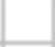
\includegraphics[max width=\textwidth]{2024_11_21_49bfa1d51da2e7fce9c5g-08}
 &  &  &  &  &  &  &  &  &  &  &  &  &  &  &  &  &  &  &  &  &  &  &  &  &  &  \\
\hline
 &  &  &  &  &  &  &  &  &  &  &  &  &  &  &  &  &  &  &  &  &  &  &  &  &  &  &  \\
\hline
 & - &  &  &  &  &  &  &  &  &  &  &  &  &  &  &  &  &  &  &  &  &  &  &  &  &  &  \\
\hline
 & \textbackslash  &  &  &  &  &  &  &  &  &  &  &  &  &  &  &  &  &  &  &  &  &  &  &  &  &  &  \\
\hline
 & - &  &  &  &  &  &  &  &  &  &  &  &  &  &  &  &  &  &  &  &  &  &  &  &  &  &  \\
\hline
 &  &  &  &  &  &  &  &  &  &  &  &  &  &  &  &  &  &  &  &  &  &  &  &  &  &  &  \\
\hline
 &  &  &  &  &  &  &  &  &  &  &  &  &  &  &  &  &  &  &  &  &  &  &  &  &  &  &  \\
\hline
 &  &  &  &  &  &  &  &  &  &  &  &  &  &  &  &  &  &  &  &  &  &  &  &  &  &  &  \\
\hline
 & - &  &  &  &  &  &  &  &  &  &  &  &  &  &  &  &  &  &  &  &  &  &  &  &  &  &  \\
\hline
 &  &  &  &  &  &  &  &  &  &  &  &  &  &  &  &  &  &  &  &  &  &  &  &  &  &  &  \\
\hline
 &  &  &  &  &  &  &  &  &  &  &  &  &  &  &  &  &  &  &  &  &  &  &  &  &  &  &  \\
\hline
 &  &  &  &  &  &  &  &  &  &  &  &  &  &  &  &  &  &  &  &  &  &  &  &  &  &  &  \\
\hline
 & - &  &  &  &  &  &  &  &  &  &  &  &  &  &  &  &  &  &  &  &  &  &  &  &  &  &  \\
\hline
 &  &  &  &  &  &  &  &  &  &  &  &  &  &  &  &  &  &  &  &  &  &  &  &  &  &  &  \\
\hline
 &  &  &  &  &  &  &  &  &  &  &  &  &  &  &  &  &  &  &  &  &  &  &  &  &  &  &  \\
\hline
\end{tabular}
\end{center}

Odpowiedź:

\begin{center}
\begin{tabular}{|c|l|c|}
\hline
\multirow{2}{*}{\begin{tabular}{c}
Wypełnia \\
egzaminator \\
\end{tabular}} & Nr zadania & 9. \\
\cline { 2 - 3 }
 & Maks. liczba pkt. & 4 \\
\cline { 2 - 3 }
 & Uzyskana liczba pkt. &  \\
\hline
\end{tabular}
\end{center}

\section*{Zadanie 10. (0-3)}
Udowodnij, że dla dowolnych liczb rzeczywistych \(x, y\) prawdziwa jest nierówność

\[
2 x^{2}+5 y^{2}-4 x y>2 x+4 y-5
\]

\begin{center}

\includegraphics[max width=\textwidth]{2024_11_21_49bfa1d51da2e7fce9c5g-09}
\end{center}

\begin{center}
\begin{tabular}{|c|l|c|}
\hline
\multirow{2}{*}{\begin{tabular}{c}
Wypełnia \\
egzaminator \\
\end{tabular}} & Nr zadania & 10. \\
\cline { 2 - 3 }
 & Maks. liczba pkt. & 3 \\
\cline { 2 - 3 }
 & Uzyskana liczba pkt. &  \\
\hline
\end{tabular}
\end{center}

\section*{Zadanie 11. (0-5)}
Przez punkt \(P=(2 ; 5)\) poprowadzono dwie proste będące stycznymi do wykresu funkcji \(f(x)=-x^{2}+6 x-7\). Wyznacz równania tych stycznych oraz współrzędne punktów styczności.\\

\includegraphics[max width=\textwidth, center]{2024_11_21_49bfa1d51da2e7fce9c5g-10}

Odpowiedź:

\begin{center}
\begin{tabular}{|c|l|c|}
\hline
\multirow{2}{*}{\begin{tabular}{c}
Wypełnia \\
egzaminator \\
\end{tabular}} & Nr zadania & 11. \\
\cline { 2 - 3 }
 & Maks. liczba pkt. & 5 \\
\cline { 2 - 3 }
 & Uzyskana liczba pkt. &  \\
\hline
\end{tabular}
\end{center}

\section*{Zadanie 12. (0-5)}
W trójkącie prostokątnym równoramiennym \(A B C\) miara \(\Varangle B\) jest równa \(90^{\circ}\). Przyprostokątna \(A B\) tego trójkąta zawiera się w prostej \(k\) o równaniu \(y=2 x+7\). Wierzchołek \(C=(2,2)\). Wyznacz współrzędne wierzchołków \(A\) oraz \(B\).\\

\includegraphics[max width=\textwidth, center]{2024_11_21_49bfa1d51da2e7fce9c5g-11}

Odpowiedź:

\begin{center}
\begin{tabular}{|c|l|c|}
\hline
\multirow{2}{*}{\begin{tabular}{c}
Wypełnia \\
egzaminator \\
\end{tabular}} & Nr zadania & 12. \\
\cline { 2 - 3 }
 & Maks. liczba pkt. & 5 \\
\cline { 2 - 3 }
 & Uzyskana liczba pkt. &  \\
\hline
\end{tabular}
\end{center}

Zadanie 13. (0-5)\\
Rozwią̇̇ nierówność \(\sqrt{x^{2}-4 x+4}+|4-x| \geq 20 \log _{32} 4\).\\

\includegraphics[max width=\textwidth, center]{2024_11_21_49bfa1d51da2e7fce9c5g-12}

Odpowiedź:

\begin{center}
\begin{tabular}{|c|l|c|}
\hline
\multirow{2}{*}{\begin{tabular}{c}
Wypełnia \\
egzaminator \\
\end{tabular}} & Nr zadania & 13. \\
\cline { 2 - 3 }
 & Maks. liczba pkt. & 5 \\
\cline { 2 - 3 }
 & Uzyskana liczba pkt. &  \\
\hline
\end{tabular}
\end{center}

Zadanie 14. (0-6)\\
Dany jest trójmian kwadratowy określony wzorem \(f(x)=(m+2) x^{2}+(3 m+1) x+3 m+1\) dla każdej liczby rzeczywistej \(x\). Wyznacz wszystkie wartości parametru m, dla których suma kwadratów dwóch różnych miejsc zerowych trójmianu \(f\) jest większa lub równa 1.\\

\includegraphics[max width=\textwidth, center]{2024_11_21_49bfa1d51da2e7fce9c5g-13}\\

\includegraphics[max width=\textwidth, center]{2024_11_21_49bfa1d51da2e7fce9c5g-14}

Odpowiedź:

\begin{center}
\begin{tabular}{|c|l|c|}
\hline
\multirow{2}{*}{\begin{tabular}{c}
Wypełnia \\
egzaminator \\
\end{tabular}} & Nr zadania & 14. \\
\cline { 2 - 3 }
 & Maks. liczba pkt. & 6 \\
\cline { 2 - 3 }
 & Uzyskana liczba pkt. &  \\
\hline
\end{tabular}
\end{center}

\section*{Zadanie 15. (0-7)}
W ostrosłup prawidłowy czworokątny o krawędzi podstawy 10 i wysokości 12 wpisano graniastosłup prawidłowy czworokątny o krawędzi podstawy \(x\) tak, że jego podstawa zawiera się w podstawie ostrosłupa, a wierzchołki drugiej podstawy należą do krawędzi bocznych tego ostrosłupa. Wyznacz pole powierzchni całkowitej tego z rozpatrywanych graniastosłupów, którego objętość jest największa.\\

\includegraphics[max width=\textwidth, center]{2024_11_21_49bfa1d51da2e7fce9c5g-15}\\

\includegraphics[max width=\textwidth, center]{2024_11_21_49bfa1d51da2e7fce9c5g-16}

Odpowiedź:

\begin{center}
\begin{tabular}{|c|l|c|}
\hline
\multirow{2}{*}{\begin{tabular}{c}
Wypełnia \\
egzaminator \\
\end{tabular}} & Nr zadania & 15. \\
\cline { 2 - 3 }
 & Maks. liczba pkt. & 7 \\
\cline { 2 - 3 }
 & Uzyskana liczba pkt. &  \\
\hline
\end{tabular}
\end{center}


\end{document}